\question{7}{8} The following shows a sequence of figures formed by dots.

\par\vspace{0.5em}
\noindent\hspace*{2em}%
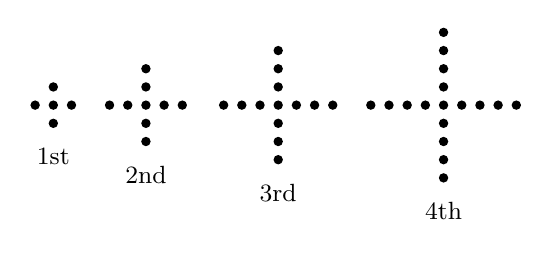
\begin{tikzpicture}[scale=0.42,baseline=-0.8ex,every node/.style={font=\small},dot/.style={circle,fill,inner sep=1.2pt}]
  \foreach \f/\x/\n in {1/0/1, 2/2.8/2, 3/6.8/3, 4/11.8/4} {
    \node[dot] at (\x,0) {};
    \foreach \k in {1,...,\n} {
      \node[dot] at (\x, \k*0.55) {};
      \node[dot] at (\x, -\k*0.55) {};
      \node[dot] at (\x+\k*0.55, 0) {};
      \node[dot] at (\x-\k*0.55, 0) {};
    }
    \ifnum\f=1 \def\flabel{1st}\fi
    \ifnum\f=2 \def\flabel{2nd}\fi
    \ifnum\f=3 \def\flabel{3rd}\fi
    \ifnum\f=4 \def\flabel{4th}\fi
    \node[below] at (\x, -\n*0.55-0.45) {\flabel};
  }
\end{tikzpicture}

\begin{subparts}
  \item Find an expression, in terms of $n$, for the number of dots in the $n$th figure.
  \item Can a figure in the sequence have $224$ dots? Explain your answer.
  \item Is the number of dots in the 11th figure odd? Explain your answer.
\end{subparts}

\answerlines{14}
